%% IMPORTANT: Once working, run latex 3 times to get listoffigures to work

%% Be sure to check spelling!

%% Put **your** name and the proper due date in place

%% Note that two of the \lstinputlisting and 
%% all of the \epsfig commands are currently commented out - until the
%% files exist, processing this code without them will result in an error
%% so leave the comments until you have created the files!

\documentclass{article}
\usepackage{amsmath}    % loads AMS-Math package
\usepackage{epsfig}     % allows PostScript files
\usepackage{listings}   % allows lstlisting environment
\usepackage{moreverb}   % allows listinginput environment
\usepackage[letterpaper, margin=0.75in]{geometry}  % set paper size/margins
\usepackage{EGR103F19}  % colorful file imports

\begin{document}
\begin{center}
\rule{6.5in}{0.5mm}\\~\\
\textbf{\large EGR 103L -- Fall 2019}\\~\\
\textbf{\huge Laboratory 2 - Introduction to Python}\\~\\
Marcus Deans (md374)\\
Lab Section 2, Tuesdays 11:45-2:35\\
15 September 2019\\~\\
{\small I understand and have adhered to all the tenets of the Duke
  Community Standard in completing every part of this assignment.  I
  understand that a violation of any part of the Standard on any part
  of this assignment can result in failure of this assignment, failure
  of this course, and/or suspension from Duke University.} 
\rule{6.5in}{0.5mm}\\
\end{center}
\tableofcontents
\listoffigures
\pagebreak

\section{Introduction}
This program displays information gathered from physical experiments regarding the relationship between force and displacement in several beams. Moreover, the experience of creating this program is designed to enhance understanding of basic Python principles. Specifically relating to springs, a model was formed based on a first-order polynomial, intended to replicate the $F=-kx$ equation that represents the relationship between spring force and displacement.
Lessons learned include:
\begin{itemize}
  \item How to create, customize, and edit graphics in Python
  \item How to save graphics for usage elsewhere
  \item How to import Python resources into a \LaTeX~ report
\end{itemize}
\section{Data Obtained}
The three data sets from the experiments are presented in Table
\ref{DataTables}.
% see handout / Pundit page for how to get formatted numbers into tables
\renewcommand{\arraystretch}{1.4}
\begin{table}[h]
\begin{center}
\begin{tabular}{ccc}
\begin{tabular}[t]{|c|c|}\hline
\multicolumn{2}{|c|}{Beam1.dat}\\ \hline
\textbf{Mass} & \textbf{Disp.}\\
(kg) & (in)\\ \hline
0 & 4.0908e-01 \\
2.4018e-01 & 5.1145e-01 \\
4.8037e-01 & 1.1085 \\
7.2055e-01 & 1.6810 \\
9.6073e-01 & 2.2016 \\
1.2009 & 2.5752 \\
1.4411 & 3.0958 \\
1.6813 & 3.5045 \\
1.9215 & 4.1159 \\
2.1616 & 4.4975 \\ \hline
\end{tabular}
&
\begin{tabular}[t]{|c|c|}\hline
\multicolumn{2}{|c|}{Beam2.dat}\\ \hline
\textbf{Mass} & \textbf{Disp.}\\
(kg) & (in)\\ \hline
         0 &  1.4446e-01 \\
2.4969e-01 & 4.5522e-02 \\
4.9939e-01 & 1.1184e-01 \\
7.4908e-01 & 2.0433e-01 \\
9.9877e-01 & 4.3890e-01 \\
1.2485 & 7.1716e-01 \\
1.4982 & 1.2029e \\
1.7479 & 1.7899 \\
1.9975 & 2.6526 \\
2.2472 & 3.7465 \\
2.4969 & 5.0663 \\ \hline
\end{tabular}
&
\begin{tabular}[t]{|c|c|}\hline
\multicolumn{2}{|c|}{Beam3.dat}\\ \hline
\textbf{Mass} & \textbf{Disp.}\\
(kg) & (in)\\ \hline
0 & 6.8650e-04 \\
3.4637e-02 & 4.3857e-02 \\
6.9273e-02 & 8.7320e-02 \\
1.0391e-01 & 1.2922e-01 \\
1.3855e-01 & 1.7391e-01 \\
1.7318e-01 & 2.1621e-01 \\
2.0782e-01 & 2.4016e-01 \\
2.4246e-01 & 2.4016e-01 \\
2.7709e-01 & 2.4016e-01 \\ \hline
\end{tabular}
\end{tabular}
\caption{Data from Three Beam Experiments \label{DataTables}}
\end{center}
\end{table}


\section{Calculation Results}
A first-order polynomial fitting algorithm determined that 
the coefficients given in Table \ref{Coefs} 
produce the best-fit of the data to a straight line.
% replace the Greek letters with your calculations
\begin{table}[h]
\begin{center}
\begin{tabular}{r|c|c}
Data File & Compliance (m/N) & Init. Disp. (m)\\ \hline \hline
\texttt{Beam1.dat} & $5.1369e-3$ & $5.7333e-3$ \\ \hline
\texttt{Beam2.dat} & $4.8048e-3$ & $-2.1624e-2$ \\ \hline
\texttt{Beam3.dat} & $2.4163e-3$ & $5.8703e-4 $ \\ \hline
\end{tabular}
\caption{Table of Compliances and Initial Displacement Values \label{Coefs}}
\end{center}
\end{table}

% \pagebreak % turn this on if it makes sense to do so by removing the first %

\section{Conclusions}
% Add your conclusions here
In conclusion, the previously measured values of displacement and the corresponding resultant force for three different beams was used to create graphical representations of the relationship for each beam. Calculations were performed in order to represent the relationship, with the graphical format providing a more accessible qualitative evaluation of the correlation between displacement and force for each beam.

Each beam appeared to, in effect, behave similarly to a spring, at least for small displacements as observed by the compliance with the graph. Beam 2 and Beam 3 were both found to have substantially higher deviation from the line of best fit compared to that of Beam 1. This may be attributable to the higher displacement that may have caused the beam to no longer act like a spring, thus no longer complying with the previously established line of best fit that held relatively true at lower displacements.

\pagebreak

\appendix
\section{Codes}
% Put the name of your file in the subsection name 
% and the listinginput input
% Be sure to include the community standard in codes!
% Add \pagebreaks if they make sense

% Note that _ in section names need \ in front (that is, \_)
% while _ in file names for lstinputlisting do not.

%%% Almost everything in this section is done; make sure you 
%%% understand how it works in general and be sure to 
%%% uncomment the lstinputlisting lines once you have created the files
\lstset{style=python103, language=python} 
\subsection{run\_beam1.m}
\lstinputlisting{run_beam1.py}
\pagebreak % this will make sure the second code is all on one page
\subsection{run\_beam2.m}
\lstinputlisting{run_beam2.py}
\pagebreak  % this will make sure the third code is all on one page
\subsection{run\_beam3.m}
\lstinputlisting{run_beam3.py}
\pagebreak  % this will start figures on a new page 
\section{Figures}
%%% Almost everything in this section is done; make sure you 
%%% understand how it works in general and be sure to 
%%% uncomment the epsfig lines once you have created the graphs
\begin{figure}[htb]
\begin{center}
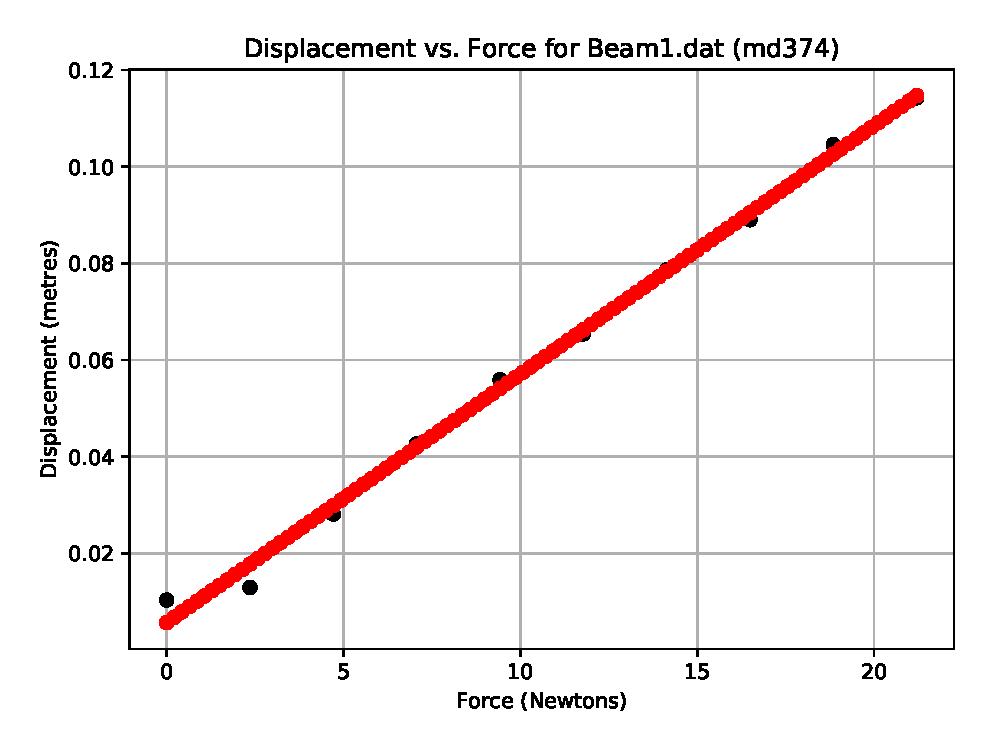
\epsfig{file=Beam1Plot.eps, width=4.5in}
\caption{Displacement vs. Force for Beam 1}
\end{center}
\end{figure}

\begin{figure}[htb]
\begin{center}
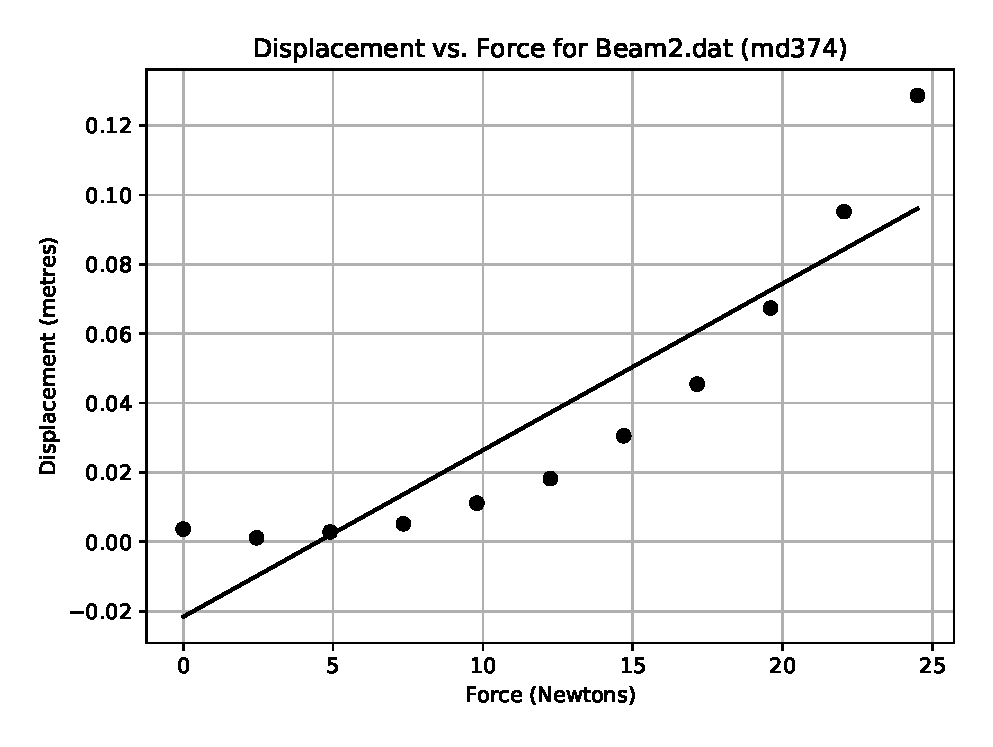
\epsfig{file=Beam2Plot.eps, width=4.5in}
\caption{Displacement vs. Force for Beam 2}
\end{center}
\end{figure}

\begin{figure}[htb]
\begin{center}
\epsfig{file=Beam3Plot.eps, width=4.5in}
\caption{Displacement vs. Force for Beam 3}
\end{center}
\end{figure}
\end{document}
